\section{Modeling}
\showtoc

\subsection{Modeling Mechanical Systems}

\begin{frame}
  \frametitle{Generalized Coordinates}
  The smallest set of coordinates that can be used to model a system is called the \blue{generalized coordinates}.
\begin{itemize}
  \item A massive particle requires three coordinates, i.e., $$\sQ \in \R^3.$$
  \item A rigid body requires six coordinates, i.e., $$\sQ \in \R^3 \times \SO = \SE.$$
\end{itemize}
Fewer coordinates can be used on systems with constraints.
\end{frame}


\begin{frame}
  \frametitle{Example: Cart with Spring}

  \only<1>{
    \begin{figure}
      \centering
      \def\svgwidth{0.8\columnwidth}
      \input{figures/cart_spring.eps_tex}
      \caption{A single coordinate, $x \in \R$, can model a cart with mass $M$ connected to a wall by a spring of stiffness $K$.}
    \end{figure}
  }

  \only<2>{
    \begin{block}{Newton's Second Law}
      By inspection, the controlled system obeys the dynamics
      \begin{align*}
        M {\ddot x} + K x = F.
      \end{align*}
      This method works on simple systems but does not scale well.
    \end{block}
    
    \begin{block}{Lagrangian Method}
      A more elegant formulation is the method of Lagrange which allows one to obtain a dynamic model by looking at the energy of a system.
    \end{block}
  }
\end{frame}

\begin{frame}
  \frametitle{Lagrangian Systems}
  Mechanical systems are defined by:
  \begin{itemize}
  \item Kinetic energy, $T : T\sQ \to \R^+$,
  \item Potential energy, $U : \sQ \to \R$,
  \end{itemize}
  which together comprise the Lagrangian,
  \begin{align*}
    \Lagrangian(q, \dot q) = T(q, \dot q) - U(q).
  \end{align*}
  Dynamical motion in such a system with external forcing $F = B(q) u$ is governed by the Euler--Lagrange equation:
  \begin{align*}
    \frac{d}{dt} \pd{\Lagrangian}{\dq} - \pd{\Lagrangian}{\q} = B(q) u.
  \end{align*}
\end{frame}

\begin{frame}
  \frametitle{Using the Lagrangian Method}
  The cart has kinetic energy $$T(x, {\dot x}) = \frac{1}{2} M {\dot x}^2$$ and potential energy $$U(x) = \frac{1}{2} K x^{2}.$$
  The Lagrangian is
  \begin{align*}
    \Lagrangian(x, {\dot x}) = \frac{1}{2} M {\dot x}^2 - \frac{1}{2} K x^{2}.
  \end{align*}
  Applying the Euler--Langrange equation gives
  \begin{align*}
    M {\ddot x} + K x = F.
  \end{align*}
\end{frame}

\begin{frame}
  \frametitle{Solutions to Continuous Systems}
  Solutions are defined as curves $$\mathscr{C} = \left\{ (c(t), {\dot c(t)}) \in T\sQ : \dot c(t) = f \circ c(t) \mbox{ and } t \in \mathscr{I} \right\}$$ parameterized by $t$ over some interval $$\mathscr{I} = [t_0, t_f].$$

  Periodic behavior implies that $$c(t) = c(t + T) \mbox{ and } {\dot c}(t) = {\dot c}(t + T)$$ for $t, t + T \in \mathscr{I}$.
\end{frame}

\begin{frame}
  \frametitle{Example: Cart with Spring}
  \only<1>{
    The time solution where $F = 0$ can be found through integration:
    \begin{align*}
      x(t) = \frac{{\dot x_{0}}}{\omega} \sin (\omega t) + x_{0} \cos (\omega t),
    \end{align*}
    where $\omega = \sqrt{k/m}$. Clearly, the solution is periodic, i.e.,
    \begin{align*}
      x(t) = x\left(t + \frac{2\pi}{\omega}\right).
    \end{align*}
    The solution to the system over one period is a \blue{limit cycle}:
    \begin{align*}
      \Omega = \left\{(x(t), \dot x(t)) \in \R^{2} : \dot x(t) = f \circ x(t) \mbox { and } t \in [0, 2\pi)\right\}.
    \end{align*}
      }
      
      \only<2>{
        \begin{figure}
          \centering
          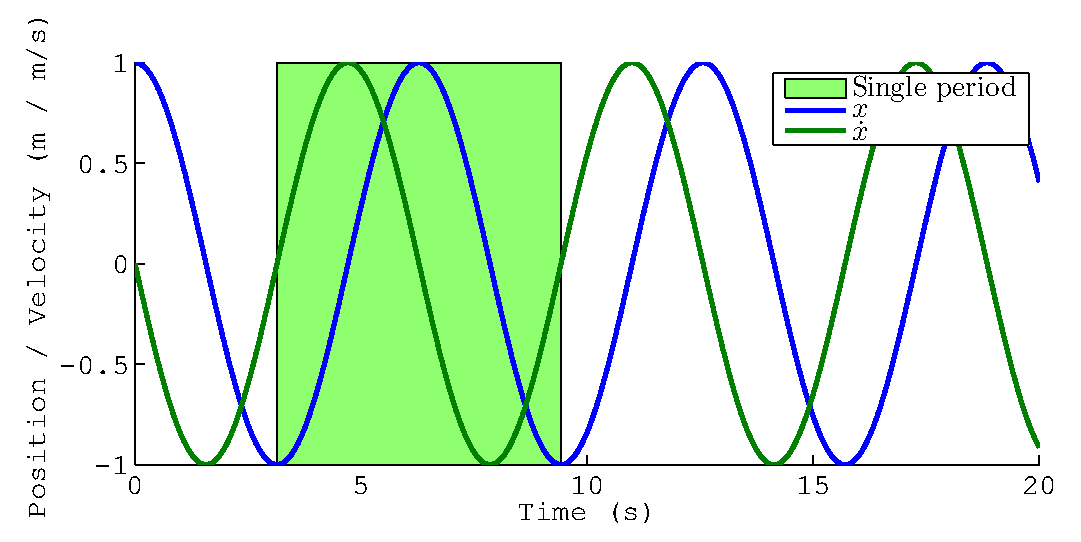
\includegraphics[width=0.8\columnwidth]{figures/cart_spring_periodic_solution}
          \caption{The cart--spring system is periodic.}
        \end{figure}
      }
\end{frame}

\begin{frame}
  \frametitle{Stability of Nonlinear Systems}
  \begin{block}{Equilibrium points}
    An equilibrium point (at the origin) is locally
    \begin{itemize}
    \item \blue{stable} if, for each $\epsilon > 0$, there exists a $\delta > 0$ s.t. $$\|x(0)\| \leq \delta  \Rightarrow \|x(t)\| \leq \epsilon,$$
      \item \blue{asymptotically stable} if stable and there exists a $\delta > 0$ s.t.
        \begin{align*}
          \|x(0)\| < \delta \Rightarrow \lim_{t \to \infty} x(t) = 0,
        \end{align*}
      \item \blue{exponentially stable} if there exist $\alpha, \delta > 0$ s.t.
        \begin{align*}
          \|x(0)\| < \delta \Rightarrow \| x(t) \| \leq \| x(0) \| e^{-\alpha t}.
        \end{align*}
    \end{itemize}
  \end{block}
\end{frame}

\begin{frame}
  \frametitle{Lyapunov's Theorem}
  Assume there exists a \blue{Lyapunov candidate function} $V(x)$ satisfying
  \begin{align*}
    V(x) \bigg\{\begin{array}{l l}
      > 0,& x \ne 0,\\
      = 0,& x = 0.
    \end{array}
  \end{align*}
  in some local region $D \subset \sX$. In $D$, the origin is locally
  \begin{itemize}
  \item \blue{stable} if, for all $x \in D$,
    \begin{align*}
      {\dot V}(x) \bigg\{\begin{array}{l l}
      \leq 0,& x \ne 0,\\
      = 0,& x = 0.
      \end{array}
    \end{align*}
  \item \blue{asymptotically stable} if, for all $x \in D$,
    \begin{align*}
      {\dot V}(x) \bigg\{\begin{array}{l l}
      < 0,& x \ne 0,\\
      = 0,& x = 0.
      \end{array}
    \end{align*}
  \end{itemize}
\end{frame}

\begin{frame}
  \frametitle{Numerical Stability Analysis}
  \begin{block}{Poincar\'e Sections}
    Consider a hyperplane transverse to the orbit,
    \begin{align*}
      \Sigma = \left\{ (q, {\dot q}) \in T\sQ : h(q, \dot q) = 0\right\}
    \end{align*}
  \end{block}
  with the appropriate scalar function $h : T\sQ \to \R$.
\end{frame}
